\documentclass{article}
\usepackage[utf8]{inputenc}
\usepackage{geometry}
\geometry{a4paper, margin=1in}
\usepackage{hyperref}
\usepackage{enumitem}
\usepackage{booktabs}
\usepackage{tikz}
\usetikzlibrary{shapes.geometric, arrows, positioning}

\title{\textbf{Chakravyuham: Automotive Intrusion Detection System}}
\author{}
\date{}

\begin{document}

\maketitle

\section{Executive Summary}
Chakravyuham is a machine learning–based Intrusion Detection System (IDS) designed to detect and classify malicious activity on in-vehicle Controller Area Network (CAN) bus systems. Modern vehicles consist of interconnected Electronic Control Units (ECUs) that communicate over CAN, a protocol that inherently lacks authentication and encryption, making it vulnerable to message injection, spoofing, and denial-of-service attacks. While existing automotive cybersecurity solutions rely heavily on rule-based detection systems, these approaches struggle to identify subtle behavioral attacks and do not generalize well across different vehicle architectures.

Our project addresses this gap by developing a behavior-driven IDS using Graph Neural Networks (GCNs) and Gradient Boosted Decision Trees (XGBoost and LightGBM), trained on real-world datasets such as the HCRL Car-Hacking and OTIDS datasets. Instead of relying on raw identifiers or dataset-specific shortcuts, our system learns communication patterns through engineered behavioral features such as inter-arrival time, entropy, transition dynamics, and graph topology representations of CAN message flows.

During development, we identified that conventional evaluation practices in IDS research often overestimate model performance due to dataset leakage and artifact memorization. This led us to redesign our training and evaluation pipeline with temporal splits, block-wise partitioning, and feature dropout mechanisms to ensure realistic performance estimation and reduce shortcut learning.

Chakravyuham ultimately proposes a more rigorous and deployable approach to automotive intrusion detection by combining behavioral machine learning, explainable feature analysis, and a deployment-aware design philosophy aimed at bridging the gap between academic IDS models and real-world in-vehicle cybersecurity systems.

\section{Threat Landscape \& Problem Statement}
Modern vehicles use the Controller Area Network (CAN) bus as the primary communication backbone between Electronic Control Units (ECUs) such as braking, engine control, infotainment, and steering systems. CAN was originally designed for reliability and efficiency in closed vehicle environments, not for security. As a result, it provides neither authentication nor encryption, meaning any node with bus access can inject or modify messages that other ECUs will blindly trust.

This fundamental design weakness makes CAN networks vulnerable to a range of real-world attacks, including Denial-of-Service (DoS) flooding, message spoofing, and fuzzy (random injection) attacks. In severe cases, attackers can impersonate critical ECUs and influence safety-critical functions such as braking or acceleration. This is not theoretical — the 2015 Jeep Cherokee remote exploitation demonstrated how external access to vehicle systems can escalate into direct control over physical vehicle behavior, highlighting the real-world consequences of CAN-level vulnerabilities.

To address these risks, automotive cybersecurity has become a regulated requirement under standards such as UN R155 and ISO/SAE 21434, pushing manufacturers to incorporate intrusion detection mechanisms within modern vehicles. However, current industrial solutions are still largely dominated by rule-based or signature-based Intrusion Detection Systems. While these approaches are efficient and certifiable for in-vehicle deployment, they rely on predefined patterns and struggle to detect unknown or evolving attack behaviors.

Machine learning–based IDS approaches offer the potential to detect subtle behavioral anomalies that rule-based systems may miss. However, their adoption in real automotive systems remains limited due to several critical challenges: lack of standardized data representation across OEMs, differences in ECU architectures and message timing across vehicles, and most importantly, the tendency of ML models to overfit dataset-specific artifacts rather than learning true attack behavior. Additionally, improper evaluation methodologies in existing research often lead to overly optimistic performance results that do not reflect real-world deployment conditions.

This creates a clear gap: while rule-based systems are deployable but limited in detection capability, machine learning systems show promise but lack reliability, generalization, and rigorous evaluation for real-world automotive deployment. Existing benchmark datasets primarily evaluate flooding, fuzzing, and spoofing-style attacks. More advanced temporal attacks such as replay attacks remain comparatively underexplored and typically require models capable of reasoning over long-term communication sequences.

Chakravyuham is built to address this gap by focusing on behavior-driven detection, leakage-resistant evaluation, and a deployment-aware ML pipeline designed specifically for realistic in-vehicle cybersecurity constraints.

\section{Solution Overview / Core Architecture}

\subsection{Pipeline overview}
Chakravyuham processes raw in-vehicle communication stream packets through a structured pipeline that abstracts low-level data frame formats into robust network-wide behavioral signatures, as illustrated in Figure~\ref{fig:pipeline_architecture}.

\begin{figure}[htbp]
\centering
\resizebox{0.9\textwidth}{!}{%
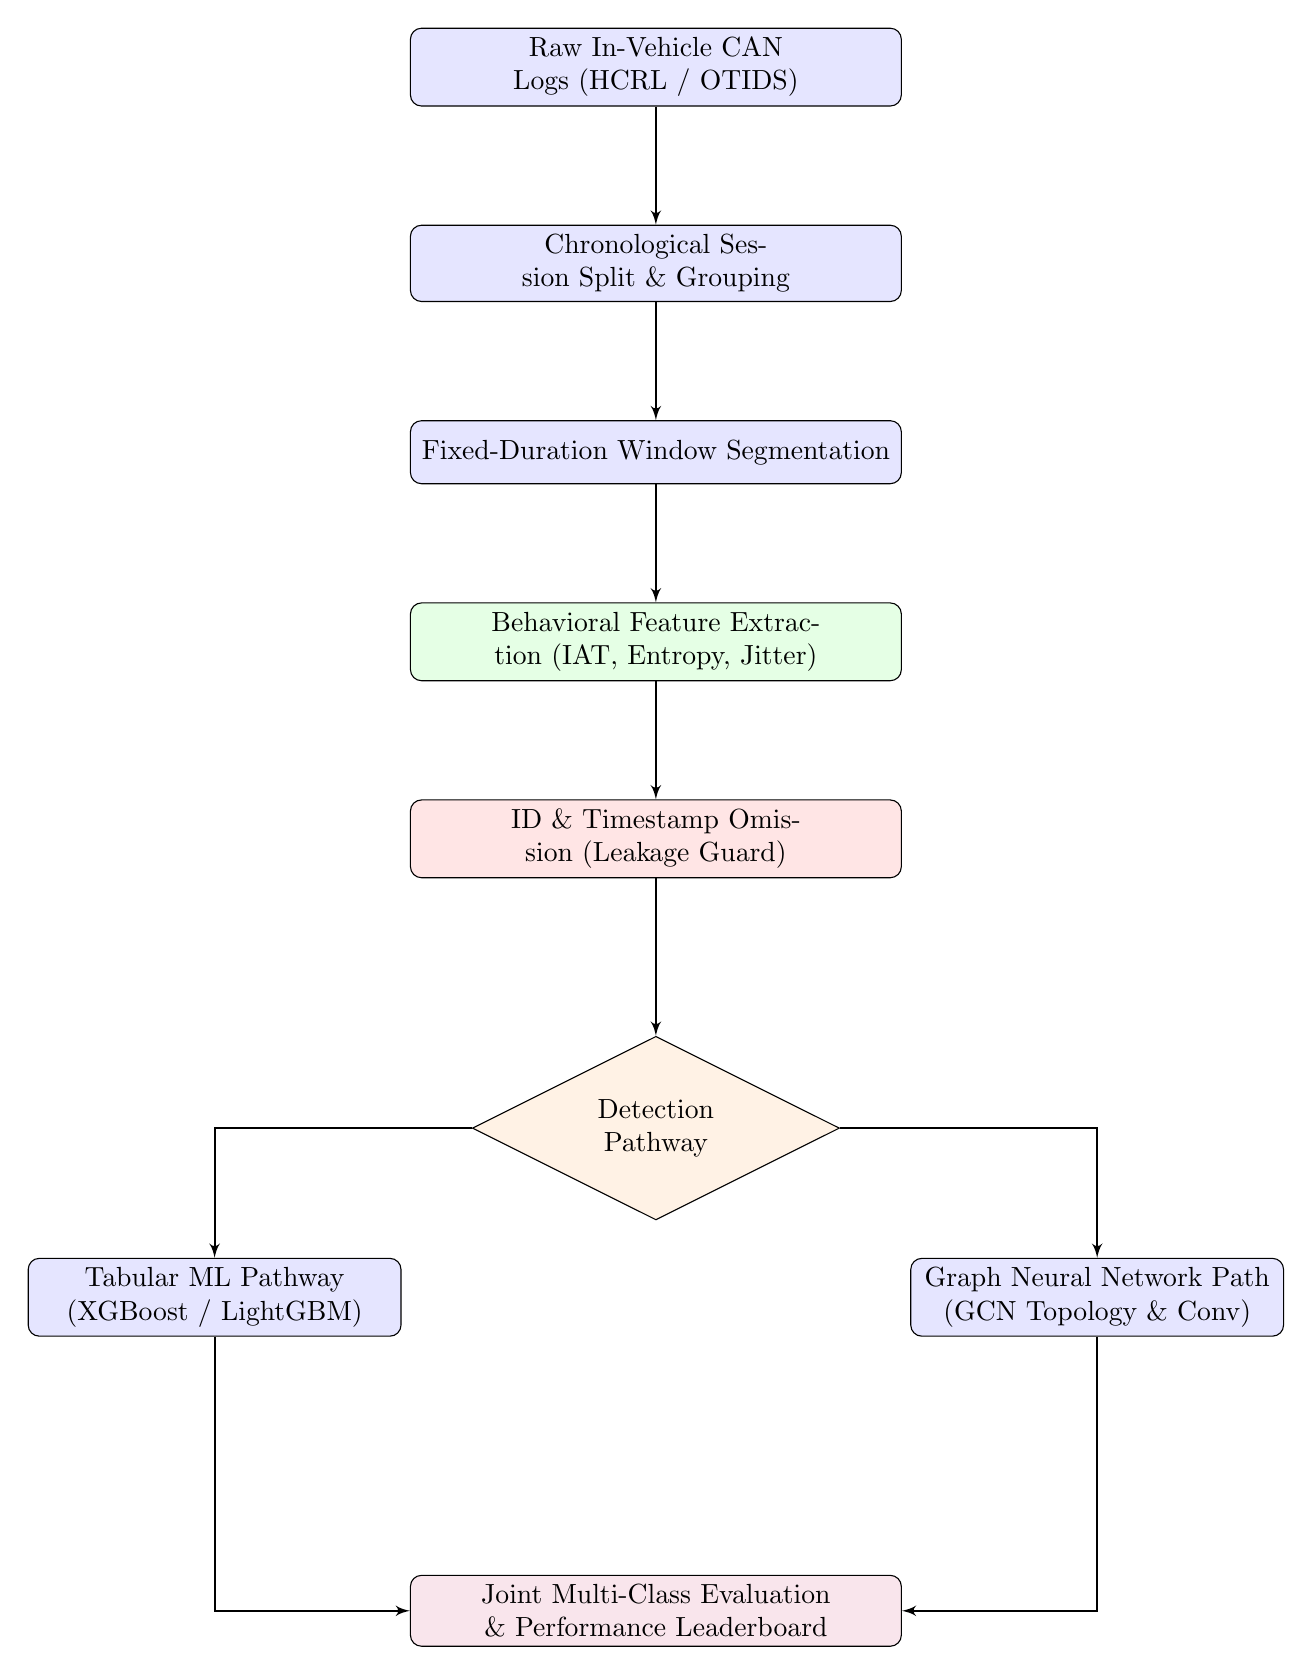
\begin{tikzpicture}[
    node distance=1.5cm,
    block/.style={rectangle, draw, fill=blue!10, text width=6cm, text centered, rounded corners, minimum height=0.8cm},
    split/.style={diamond, draw, fill=orange!10, text width=2.5cm, text centered, aspect=2, minimum height=0.8cm},
    line/.style={draw, -latex', thick}
]
    % Nodes
    \node (raw) [block] {Raw In-Vehicle CAN Logs (HCRL / OTIDS)};
    \node (prep) [block, below=of raw] {Chronological Session Split \& Grouping};
    \node (wind) [block, below=of prep] {Fixed-Duration Window Segmentation};
    \node (feat) [block, fill=green!10, below=of wind] {Behavioral Feature Extraction (IAT, Entropy, Jitter)};
    \node (excl) [block, fill=red!10, below=of feat] {ID \& Timestamp Omission (Leakage Guard)};
    
    \node (choice) [split, below=of excl, yshift=-0.5cm] {Detection Pathway};
    
    \node (tab) [block, below left=of choice, xshift=-1cm, text width=4.5cm] {Tabular ML Pathway\\(XGBoost / LightGBM)};
    \node (graph) [block, below right=of choice, xshift=1cm, text width=4.5cm] {Graph Neural Network Path\\(GCN Topology \& Conv)};
    
    \node (eval) [block, below=of choice, yshift=-3cm, fill=purple!10] {Joint Multi-Class Evaluation \& Performance Leaderboard};

    % Connections
    \draw [line] (raw) -- (prep);
    \draw [line] (prep) -- (wind);
    \draw [line] (wind) -- (feat);
    \draw [line] (feat) -- (excl);
    \draw [line] (excl) -- (choice);
    \draw [line] (choice) -| (tab);
    \draw [line] (choice) -| (graph);
    \draw [line] (tab) |- (eval);
    \draw [line] (graph) |- (eval);
\end{tikzpicture}
}
\caption{Chakravyuham Intrusion Detection System Data and Processing Pipeline}
\label{fig:pipeline_architecture}
\end{figure}

\subsubsection{1. CAN Data Ingestion}
\begin{itemize}[noitemsep]
    \item Raw CAN traffic is collected from the HCRL Car-Hacking and OTIDS datasets.
    \item Each HCRL attack file is an \textbf{independent recording session} with its own timestamp origin.
    \item Sessions are processed independently to preserve chronological communication patterns.
    \item Files are \textbf{never shuffled together}, since they represent separate recordings on different clocks.
    \item Dataset combination occurs only after preprocessing/feature extraction where appropriate, preventing artificial temporal mixing.
\end{itemize}

\subsubsection{2. Time-Based Windowing}
\begin{itemize}[noitemsep]
    \item Continuous CAN traffic is segmented into \textbf{fixed-duration time windows}.
    \item Each window captures a short behavioural snapshot of vehicle communication.
    \item Time-based windows were chosen instead of count-based windows because CAN traffic density varies with vehicle state; fixed-duration windows preserve consistent temporal context for learning.
    \item Session-aware splitting preserves chronology and prevents train-test leakage.
    \item Unlike conventional random frame-level train/test splitting, chronological block-wise partitioning prevents temporally adjacent CAN frames from appearing in both training and evaluation. Since CAN traffic exhibits strong temporal correlation, this produces a substantially more realistic estimate of deployment performance and reduces leakage-driven optimism.
\end{itemize}

\subsubsection{3. Behavioural Feature Extraction}
Instead of relying on raw CAN identifiers, Chakravyuham represents every communication window using behavioural descriptors that capture \textbf{how the network behaves} rather than \textbf{which ECU transmitted the message}. The chosen features were selected because they remain meaningful across different vehicles and attack scenarios, whereas raw identifiers often encode vehicle-specific information that does not generalize.

The features are grouped according to the type of behaviour they capture.

\paragraph{Traffic Behaviour}
\begin{itemize}[noitemsep]
    \item \textbf{Message Frequency} – Number of messages transmitted by an ECU within a time window. Flooding attacks such as DoS typically produce abnormal transmission rates.
    \item \textbf{Inter-Arrival Time (IAT)} – Time elapsed between consecutive transmissions from an ECU. Captures timing abnormalities introduced by injected traffic.
    \item \textbf{Timing Jitter} – Variation in inter-arrival times. Identifies disruption to otherwise periodic CAN communication.
    \item \textbf{Burstiness} – Measures whether messages arrive in sudden bursts or at a relatively uniform rate, helping distinguish coordinated attacks from normal traffic.
\end{itemize}

\paragraph{Payload Behaviour}
\begin{itemize}[noitemsep]
    \item \textbf{Payload Entropy} – Measures the randomness of payload bytes. Random injection attacks (e.g., Fuzzy attacks) generally exhibit much higher entropy than legitimate traffic.
    \item \textbf{Payload Hamming Distance} – Measures the number of bit changes between consecutive payloads of the same message. Detects sudden abnormal payload variations while remaining independent of the actual payload value.
\end{itemize}

\paragraph{Communication Behaviour}
\begin{itemize}[noitemsep]
    \item \textbf{Transition Entropy} – Quantifies the uncertainty of communication transitions between ECUs. Malicious injections often alter normal communication sequences, increasing transition randomness.
    \item \textbf{ECU Communication Statistics} – Capture how individual ECUs interact with the rest of the network through message exchange patterns.
    \item \textbf{Graph Topology Metrics (GCN pathway)} – Describe the structural organization of the communication graph, allowing graph-based models to detect relational anomalies rather than isolated message anomalies.
\end{itemize}

\paragraph{Leakage Prevention}
A fundamental design decision is to remove features that allow shortcut learning.
The following are \textbf{never} used as predictive features:
\begin{itemize}[noitemsep]
    \item Raw CAN arbitration IDs
    \item Raw timestamps
    \item Attack start positions
    \item Window indices
    \item Message indices
    \item Other positional dataset information
\end{itemize}
This forces every model to learn behavioural patterns instead of memorizing dataset artifacts.

\subsubsection{4. Statistical ML Pipeline}
Instead of learning directly from raw CAN traffic, the statistical pipeline operates on the engineered behavioural feature vector extracted from each time window. Each window is represented by timing, payload and communication statistics that summarize the behaviour of the network during that short interval. These features are then supplied independently to multiple tree-based ensemble models, including Random Forest, XGBoost and LightGBM.

Rather than committing to a single model family, Chakravyuham evaluates each architecture independently to understand its detection capability, robustness against dataset artifacts, computational requirements and suitability for deployment on resource-constrained automotive hardware.

Tree-based ensemble methods were selected because they provide several practical advantages for embedded intrusion detection, including fast inference, low memory requirements, straightforward explainability through feature importance analysis, and efficient deployment using compiled inference libraries such as Treelite or m2cgen.

Each trained model produces a window-level prediction indicating whether the observed behaviour corresponds to normal vehicle communication or one of the supported attack categories. The resulting models are then compared using both conventional benchmark metrics and the leakage-aware evaluation methodology developed during this project.

\subsubsection{5. Graph Neural Network Pipeline}
Instead of treating each CAN message in isolation, the GCN pathway represents every window as a communication graph, allowing the model to learn structural relationships between ECUs rather than just per-message statistics.

\paragraph{Graph Construction}
\begin{itemize}[noitemsep]
    \item Each unique CAN arbitration ID within a window becomes a graph node.
    \item A directed edge is created for every transition between two consecutive CAN messages, representing which ID communicated after which.
    \item Repeated transitions between the same pair of IDs are accumulated into a single edge weight rather than creating duplicate edges, capturing how strong or frequent that communication pattern is within the window.
    \item Self-loops are retained to preserve repetitive communication behaviour commonly seen in CAN networks, where the same ID can transmit consecutively.
    \item If a window happens to produce no repeated transitions between distinct IDs, the graph falls back on self-loops so the convolution still has neighbouring structure to aggregate over.
\end{itemize}

\paragraph{Node-Level Features}
\begin{itemize}[noitemsep]
    \item Each node carries 11 behavioural and statistical descriptors of that arbitration ID's activity within the window (drawn from the traffic, payload, and communication behaviour groups described above), rather than the ID itself.
    \item Each arbitration ID's typical behaviour is tracked over time, and features are expressed as how much a window deviates from that ID's usual pattern, rather than as raw values. This lets the model spot what looks abnormal for that specific ID, instead of relying on fixed thresholds.
\end{itemize}

\paragraph{Graph Convolutional Network Architecture}
\begin{itemize}[noitemsep]
    \item The graph is passed through two stacked graph convolution layers: GCNConv (11 $\rightarrow$ 8) followed by a ReLU activation, then GCNConv (8 $\rightarrow$ 8) followed by another ReLU activation.
    \item Each layer lets a node update its representation by aggregating information from its neighbouring nodes and the edges connecting them, so the model learns structural and relational patterns, such as unusual transition behaviour or abnormal connectivity, rather than relying on any single node's features in isolation.
\end{itemize}

\paragraph{Pooling}
\begin{itemize}[noitemsep]
    \item After the convolution layers, node-level embeddings are aggregated into a single fixed-length graph-level representation using global mean pooling.
    \item This produces one summary representation per window, combining the behaviour of every ECU present in that window into a form suitable for classification.
\end{itemize}

\paragraph{Graph-Level Features}
\begin{itemize}[noitemsep]
    \item Beyond the pooled node representation, global features describing the overall structure of the window's communication graph are computed separately, such as the number of distinct IDs present, the entropy of transitions across the whole graph, and the overall connectivity density of the graph.
    \item These global features are only added in after pooling, so the individual ECU behaviour captured by each node and the overall structure of the communication graph are kept separate until the final step, rather than being blended together too early.
\end{itemize}

\paragraph{Classifier}
\begin{itemize}[noitemsep]
    \item Dropout is applied before the final classification layer, randomly deactivating part of the combined representation during training so the model doesn't over-rely on any single feature or pathway, helping prevent overfitting.
    \item A final linear layer maps this representation to the attack categories being predicted, producing the window's classification.
\end{itemize}

\subsection{Key Design Philosophy}
A core objective throughout Chakravyuham is to ensure that the models learn \textbf{behavioural characteristics of CAN traffic rather than memorizing dataset-specific patterns}.

To achieve this, we deliberately exclude features that could act as shortcuts, including raw timestamps, attack start positions, message indices, window positions, and other positional information. Similarly, raw CAN arbitration IDs are never used as predictive features. In the statistical ML pipeline they are transformed into behavioural statistics, while in the GCN they are used only to define graph structure (node identity and communication transitions), never as feature values.

This forces the models to learn \textbf{how ECUs communicate, how their behaviour changes over time, and how interactions between ECUs evolve}, instead of simply recognizing identifiers or dataset artifacts. This design philosophy was established after our leakage investigation revealed that models could achieve unrealistically high benchmark performance by exploiting dataset-specific shortcuts rather than genuine behavioural signals. Every subsequent improvement proposed in Chakravyuham is built around preventing shortcut learning and encouraging robust behavioural understanding.

\subsection{What Makes This Architecture Different}
Unlike conventional benchmark-driven IDS research, Chakravyuham is designed around \textbf{deployment-oriented engineering} rather than maximizing dataset accuracy alone.

\textbf{Leakage-aware evaluation}
\begin{itemize}[noitemsep]
    \item Temporal and block-wise dataset partitioning instead of purely random sampling.
    \item Reduces overly optimistic performance caused by frame-level correlations and dataset leakage.
\end{itemize}

\textbf{Behaviour-first feature engineering}
\begin{itemize}[noitemsep]
    \item Models learn timing behaviour, payload evolution and communication patterns instead of memorizing identifiers or dataset artifacts.
    \item Improves robustness and forms the basis for future cross-vehicle generalization.
\end{itemize}

\textbf{Comparative architecture evaluation}
\begin{itemize}[noitemsep]
    \item Rather than assuming one machine learning model is optimal, Chakravyuham systematically evaluates tree-based ensemble methods and Graph Neural Networks to understand their respective strengths, limitations and deployment feasibility.
    \item This enables architecture selection to be driven by engineering evidence rather than benchmark popularity.
\end{itemize}

\textbf{Deployment-oriented design}
\begin{itemize}[noitemsep]
    \item Prioritizes lightweight models suitable for embedded automotive hardware.
    \item Considers inference latency, memory footprint and edge deployment from the earliest stages of development rather than as an afterthought.
\end{itemize}


\section{Engineering Challenges \& Methodology Evolution}
Chakravyuham was not developed as a static pipeline but evolved through multiple iterative stages of experimentation, evaluation, and correction. While initial baselines showed strong benchmark performance on standard evaluation setups, deeper investigation revealed that many of these results were influenced by dataset artifacts, leakage patterns, and shortcut learning rather than true behavioral understanding of CAN bus traffic. This section outlines the key engineering discoveries that shaped the final methodology.

\subsection{Initial Baseline and Hidden Optimism}
The first version of the system was trained using standard machine learning pipelines on the HCRL Car-Hacking dataset with conventional preprocessing and random frame-level train-test splits. This setup represented the initial developer baseline. Early results showed extremely high performance, with classifications matching or exceeding \textbf{99.98\% accuracy} and \textbf{99.96\% Macro F1} scores across attack classes.

However, subsequent investigations revealed that this baseline performance was over-optimistic. Frame-level random shuffling allowed packets from the same millisecond attack burst to be split across training and test sets, resulting in severe temporal leakage. Additionally, TreeSHAP explainability analyses showed that the models were not learning actual anomalous network behaviors but were simply memorizing vehicle-specific CAN arbitration IDs as direct mapping rules. Under out-of-session validation or simulated ID-spoofed adversarial traffic, the baseline models collapsed, indicating that the high accuracy was an artifact of dataset representation rather than genuine intrusion detection capability.

\subsection{Discovery of Dataset Leakage and Shortcut Learning}
A detailed error analysis revealed that the model was exploiting unintended signals:
\begin{itemize}[noitemsep]
    \item \textbf{CAN ID leakage:} certain attack types consistently reused specific arbitration IDs, allowing models to memorize attack identity rather than behavior
    \item \textbf{Temporal proximity leakage:} adjacent frames within the same attack burst were being split across train/test sets, inflating performance
    \item \textbf{Timestamp dependence:} early features inadvertently encoded positional information within logs
\end{itemize}
This led to a key realization:
High accuracy was not necessarily equivalent to true intrusion detection capability. These findings demonstrated that evaluation methodology, rather than model architecture, was the primary factor affecting reported performance, necessitating a redesign of the data handling and training pipeline.

To validate this, we introduced stricter evaluation methods, which immediately exposed significant performance degradation in certain attack categories (especially RPM spoofing), confirming that earlier results were not fully reliable.

\subsection{Methodological Corrections}
Taking into account critical problems we found such as data leakage and evaluation bias, we progressively redesigned the pipeline around leakage-resistant principles. Rather than optimizing solely for benchmark accuracy, every methodological change was evaluated based on whether it improved the credibility of real-world deployment performance. These are the decisions we came to:
\begin{itemize}[noitemsep]
    \item \textbf{Block-wise temporal splitting:} CAN logs were segmented into fixed windows and split chronologically to prevent leakage across adjacent frames
    \item \textbf{Seeded shuffled block partitioning:} ensured all attack classes were fairly represented in train/validation/test splits without introducing temporal overlap
    \item \textbf{Removal of raw positional features:} timestamps, message indices, and session position were excluded as direct features
\end{itemize}
This shifted the model from learning \textit{where an attack occurs} to \textit{how an attack behaves}.

\subsection{Synthetic augmentation + failure insight}
A major limitation identified during development was \textbf{extreme class imbalance}, where normal traffic dominates the dataset and certain attack types are underrepresented. This resulted in models that were biased toward predicting normal behavior, with weak recall on minority attack classes.

To address this, we experimented with:
\begin{itemize}[noitemsep]
    \item Oversampling underrepresented attack classes
    \item Synthetic augmentation of attack windows
    \item Controlled balancing of training distributions
\end{itemize}

\textbf{Key finding:}
Performance improvements were observed only when the model was exposed to a sufficiently balanced representation of attack behaviors. This confirmed that the issue was not model incapability, but \textbf{insufficient learning exposure for minority classes}.

However, the experiments also highlighted an important constraint:
Blind or uncontrolled synthetic generation can distort the true distribution of CAN bus behavior and degrade model reliability.

\subsubsection{Key Constraints for Synthetic Data in CAN IDS}
From these experiments, we derived important principles for synthetic data generation:
\begin{itemize}[noitemsep]
    \item Synthetic samples must preserve \textbf{temporal structure of attack bursts}, not just individual frames
    \item Window-level consistency is critical — attacks are behavior sequences, not isolated messages
    \item Class balance must be improved without breaking natural traffic distribution ratios
    \item Feature-level distributions (entropy, IAT, frequency) must remain aligned with real attack statistics
    \item Synthetic augmentation must be constrained within realistic operational ranges to avoid distribution drift
\end{itemize}

\subsubsection{Pipeline Insight: Real + Synthetic Separation Strategy}
Based on these findings, we structured the data pipeline conceptually as:
\begin{itemize}[noitemsep]
    \item \textbf{Dataset A (Real CAN Traffic)} $\rightarrow$ Feature extraction $\rightarrow$ baseline behavioral modeling
    \item \textbf{Dataset B (Synthetic / Augmented Attack Windows)} $\rightarrow$ Controlled feature generation respecting temporal and statistical constraints
    \item \textbf{Merging Stage} $\rightarrow$ Feature-level alignment and normalization before training
\end{itemize}
This reinforced a key insight:
Synthetic data is only useful when it reinforces real behavioral structure — not when it attempts to approximate raw signal generation.

\subsubsection{Core Conclusion from This Phase}
This phase demonstrated that the primary limitation in early models was not architectural or algorithmic, but data exposure imbalance. The model was capable of learning attack behaviour, but required sufficient and well-structured examples of minority attack classes to do so effectively.

This investigation fundamentally changed our perspective on synthetic augmentation. Rather than treating it as simple oversampling, we now view it as a controlled behavioural data generation process that must preserve temporal structure, statistical consistency, and realistic attack dynamics. This directly informs the synthetic augmentation pipeline described in the future roadmap.

\subsection{Feature Design Reorientation (From Identity to Behaviour)}
One of the most critical changes in the project was redefining feature philosophy.
We observed that including raw identifiers (like CAN IDs) as direct features led to:
\begin{itemize}[noitemsep]
    \item Overfitting to ECU identity
    \item Poor adversarial robustness (especially under spoofing)
    \item Failure under cross-session evaluation
\end{itemize}

However, removing them entirely caused:
\begin{itemize}[noitemsep]
    \item Loss of ECU-level behavioral anchoring
    \item Increased false positives in certain configurations
\end{itemize}

This led to a controlled compromise:
\begin{itemize}[noitemsep]
    \item CAN IDs were retained only as \textbf{graph structure identifiers}, not learning features
    \item Feature learning was shifted entirely to \textbf{behavioral signals}, such as:
    \begin{itemize}[noitemsep]
        \item inter-arrival time statistics
        \item entropy-based payload variation
        \item transition dynamics between ECUs
        \item rolling Z-score deviations from historical baselines
    \end{itemize}
\end{itemize}
This transition was central in converting the system from a \textbf{pattern memorizer to a behavioral anomaly detector}.

\subsection{Feature Dropout and Overfitting Control}
Further experiments showed that even behavioral models could overfit when feature visibility was unrestricted.

To counter this, we introduced:
\begin{itemize}[noitemsep]
    \item \textbf{Feature dropout (column subsampling)} in GBDT models
    \item Controlled exposure of CAN ID-related structure during training
    \item Constraints on tree depth and feature influence
\end{itemize}

This created a balance between:
\begin{itemize}[noitemsep]
    \item learning ECU identity relationships (useful for detection)
    \item avoiding deterministic memorization of attack signatures
\end{itemize}


\section{Evaluation Results \& Model Benchmarks}
We evaluated the candidate models (XGBoost, LightGBM, Random Forest, GCNIDS, and MosaicCNN) across the HCRL (Car-Hacking) and OTIDS datasets under two distinct feature configurations:
\begin{enumerate}
    \item \textbf{Basic Feature Set}: Retains raw arbitration IDs and DLC values as tabular inputs (15 features).
    \item \textbf{Advanced Feature Set}: Excludes all raw identifiers and DLC values, utilizing only engineered behavioral metrics (frequency, IAT, timing jitter, payload entropy, and payload Hamming distance) to ensure spoofing immunity (5 features).
\end{enumerate}

To ensure realistic performance estimation and prevent temporal proximity leakage, the evaluation was conducted using a strict chronological block-wise temporal split (10-second segment grouping).

\begin{table}[htbp]
\centering
\caption{Comprehensive Model Performance Leaderboard}
\label{tab:comprehensive_results}
\resizebox{\textwidth}{!}{%
\begin{tabular}{lllccccc}
\toprule
\textbf{Dataset} & \textbf{Model} & \textbf{Feature Set} & \textbf{Accuracy (\%)} & \textbf{Macro F1 (\%)} & \textbf{FPR (\%)} & \textbf{Latency (ms)} & \textbf{Size (MB)} \\ 
\midrule
\textbf{OTIDS} & XGBoost & Basic & 87.9923 & 56.2686 & 12.8036 & 0.382 & 0.5417 \\
 & LightGBM & Basic & 88.9404 & 64.2521 & 10.4034 & 1.186 & 0.6011 \\
 & RandomForest & Basic & 87.6322 & 54.4405 & 13.2490 & 1.872 & 1.5301 \\
 & GCNIDS & Basic & 82.3962 & 54.3648 & 11.2650 & 11.280 & 0.0033 \\
 & MosaicCNN & Basic & 79.4073 & 38.5910 & 15.7168 & 1.480 & 0.7370 \\ 
\cmidrule{2-8}
 & XGBoost & Advanced & 87.4272 & 54.8457 & 13.2979 & 0.387 & 0.6934 \\
 & \textbf{LightGBM} & \textbf{Advanced} & \textbf{89.5582} & \textbf{66.3019} & \textbf{10.5303} & \textbf{1.181} & \textbf{0.6814} \\
 & RandomForest & Advanced & 86.7896 & 50.3871 & 14.1487 & 2.102 & 2.1906 \\
 & GCNIDS & Advanced & 83.9139 & 60.7933 & 9.1778 & 10.937 & 0.0033 \\
 & MosaicCNN & Advanced & 79.4453 & 38.6627 & 15.7565 & 1.524 & 0.7370 \\ 
\midrule
\textbf{HCRL} & XGBoost & Basic & 99.9966 & 99.9904 & 0.0038 & 0.401 & 0.4593 \\
 & LightGBM & Basic & 99.9996 & 99.9988 & 0.0004 & 1.252 & 0.9055 \\
 & RandomForest & Basic & 99.9725 & 99.9235 & 0.0334 & 1.726 & 0.7034 \\
 & GCNIDS & Basic & 66.8967 & 56.9251 & 0.0184 & 10.115 & 0.0033 \\
 & MosaicCNN & Basic & 68.0626 & 57.7610 & 0.1726 & 1.508 & 0.7375 \\ 
\cmidrule{2-8}
 & XGBoost & Advanced & 99.9280 & 99.8312 & 0.0845 & 0.422 & 0.6164 \\
 & \textbf{LightGBM} & \textbf{Advanced} & \textbf{99.9959} & \textbf{99.9903} & \textbf{0.0039} & \textbf{0.923} & \textbf{0.8525} \\
 & RandomForest & Advanced & 99.9687 & 99.9265 & 0.0369 & 1.745 & 1.1600 \\
 & GCNIDS & Advanced & 66.7275 & 56.7959 & 0.0084 & 10.308 & 0.0033 \\
 & MosaicCNN & Advanced & 66.8304 & 53.5868 & 0.6713 & 1.498 & 0.7375 \\ 
\bottomrule
\end{tabular}%
}
\end{table}

\subsection{Key Observations \& Discussion}
\begin{itemize}
    \item \textbf{Adversarial Robustness and Signal Cleanliness}: In tree-based models, the omission of raw CAN ID and DLC values in the Advanced feature set did not degrade performance. In fact, LightGBM saw its Macro F1 on OTIDS improve from \textbf{64.25\% to 66.30\%}. This indicates that excluding raw indices prevents tree-based splits from overfitting to categorical noise and forces them to align on true physical timing indicators.
    \item \textbf{Deep Learning Windowing Performance Degradation}: Both GCNIDS and MosaicCNN exhibit lower Macro F1 metrics (averaging ~66\% on HCRL) compared to gradient-boosted trees. Since deep learning classifications are computed over aggregated temporal windows, sparse attacks (such as spoofing commands hidden within dense normal sequences) get blurred. When window-level outputs are spread back to frame granularities, normal background messages within the attack window trigger false positives.
    \item \textbf{Resource and Execution Benchmarks}: Tree models compiled for inference exhibit exceptional latency properties. XGBoost leads with \textbf{0.38 ms} per window inference. GCNIDS represents the slowest path with \textbf{10.9 ms} of execution time due to graph-construction overhead, but presents the smallest footprint for memory footprint storage (\textbf{0.0033 MB}).
\end{itemize}


\section{Industry Landscape \& Remaining Challenges}
\subsection{Commercial Solutions}
The automotive cybersecurity landscape is currently dominated by a small number of Tier-1 security vendors, primarily operating under regulatory constraints such as \textbf{UN R155} and \textbf{ISO/SAE 21434}, which mandate intrusion detection, incident response, and fleet-level monitoring.

\textbf{Bosch ETAS (ESCRYPT)} is one of the most widely deployed solutions:
\begin{itemize}[noitemsep]
    \item \textbf{CycurIDS-CAN} performs CAN intrusion detection using deterministic, rule-based logic generated from OEM vehicle network specifications.
    \item \textbf{CycurIDS-M} aggregates detected security events into a centralized Security Event Management system for fleet-level analysis.
    \item \textbf{CycurGATE} extends protection to automotive Ethernet through hardware-accelerated firewalling and packet inspection at line speed.
\end{itemize}

\textbf{PlaxidityX (Argus Cyber Security)} implements a Vehicle Detection and Response (VDR) framework:
\begin{itemize}[noitemsep]
    \item Software-based IDPS for CAN intrusion detection using timing and behavioral rules
    \item Gateway/ECU-level deployment for in-vehicle monitoring
    \item Hardware-based \textbf{vDome}, which uses ECU electrical fingerprinting for physical-layer attack detection
\end{itemize}

\subsection{Current Industry Approach}
Across both companies, the dominant design pattern is:
\begin{itemize}[noitemsep]
    \item \textbf{Rule-based detection on vehicle}
    \item \textbf{Signature/heuristic systems for known behaviors}
    \item \textbf{Cloud / VSOC-based analytics for fleet intelligence}
\end{itemize}
Machine learning is generally not deployed as the primary in-vehicle detection mechanism.

\subsection{Why the Industry Avoids Heavy ML On-Vehicle}
This design choice is driven by practical automotive constraints:
\begin{itemize}[noitemsep]
    \item \textbf{Deterministic execution requirements} (predictable behavior required for safety certification under ISO 26262)
    \item \textbf{Limited ECU compute and memory budgets}
    \item \textbf{Real-time latency constraints}
    \item \textbf{Availability of OEM network specifications enabling rule generation}
    \item \textbf{Hard problem of cross-vehicle generalization (no standard representation across OEMs)}
\end{itemize}
As a result, ML is often reserved for \textbf{off-vehicle analytics (VSOC / cloud)} rather than real-time in-vehicle detection.

\subsection{Remaining Gaps in Existing Systems}
Despite maturity in rule-based systems, several key limitations remain:
\begin{itemize}[noitemsep]
    \item \textbf{Behavioral attacks are hard to generalize with rules} (subtle timing drift, impersonation patterns)
    \item \textbf{Limited cross-vehicle generalization} due to OEM-specific configurations
    \item \textbf{High dependency on manual rule engineering per vehicle model}
    \item \textbf{Weak handling of unseen attack variations}
    \item \textbf{Evaluation bias due to dataset artifacts in ML-based research systems}
    \item \textbf{No unified, scalable learning-based representation of CAN behavior}
\end{itemize}

This creates a clear gap between:
\begin{itemize}[noitemsep]
    \item Highly deployable but rigid rule-based systems \\
    vs
    \item Flexible but non-deployable ML-based research systems
\end{itemize}

\subsection{Where Chakravyuham Fits}
Chakravyuham is positioned at the intersection of these two paradigms:
\begin{itemize}[noitemsep]
    \item Retains \textbf{deterministic deployability principles} (edge-feasible, low-latency models)
    \item Introduces \textbf{behavioral machine learning over rule systems}
    \item Moves away from raw CAN ID dependence toward \textbf{structured behavioral representation}
    \item Designs for \textbf{deployment realism rather than benchmark optimization}
\end{itemize}

This directly addresses the gap between industrial rule-based systems and academic ML-based IDS models by focusing on:
\begin{itemize}[noitemsep]
    \item Real-time feasibility
    \item Cross-vehicle adaptability (via structured representations like VSS directionally)
    \item Robust behavioral learning instead of dataset memorization
\end{itemize}

\section{Future Roadmap}
This roadmap is derived directly from limitations observed during model development, evaluation, and adversarial testing. Each component targets a specific failure mode identified in dataset behavior, model generalization, or deployment constraints.

Rather than adding standalone features, this section outlines the \textbf{engineering steps required to transition from a high-performing prototype to a deployment-ready automotive intrusion detection system}.

\subsection{Dataset Dependence $\rightarrow$ Synthetic Attack Augmentation Engine}
A key limitation in IDS research, including our experiments, is that high benchmark performance often results from \textbf{dataset-specific artifacts rather than true behavioral learning}. In structured datasets like HCRL, attack patterns can contain exploitable shortcuts that models memorize instead of generalizing behavior.

\textbf{Proposed Solution}
We introduce a synthetic augmentation framework that:
\begin{itemize}[noitemsep]
    \item Generates controlled variations of:
    \begin{itemize}[noitemsep]
        \item DoS flooding patterns
        \item Fuzzy injection behavior
        \item Impersonation-style payload drift
    \end{itemize}
    \item Preserves CAN temporal integrity:
    \begin{itemize}[noitemsep]
        \item message ordering consistency
        \item inter-arrival timing structure
        \item per-ID communication dynamics
    \end{itemize}
    \item Balances underrepresented attack classes to reduce skewed learning
\end{itemize}

\textbf{Objective}
Replace dataset shortcuts with \textbf{behaviorally diverse attack representations}, improving robustness beyond benchmark conditions.

\subsection{OEM Dependence $\rightarrow$ Standardized Signal Abstraction (VSS-Driven, Conditional)}
A major barrier in real-world deployment is that CAN-based IDS models are tightly coupled to \textbf{OEM-specific CAN IDs and message formats}, limiting cross-vehicle transferability.

\textbf{Proposed Solution}
We were inspired by the growing industry adoption of the \textbf{COVESA Vehicle Signal Specification (VSS)} and chose to adopt it as a normalization layer:
\begin{itemize}[noitemsep]
    \item Maps raw CAN IDs to standardized signal representations
    \item Enables learning over signal semantics instead of vendor-specific identifiers
    \item Allows architecture reuse across OEMs without redesign
\end{itemize}

\textbf{Feasibility Constraint}
\begin{itemize}[noitemsep]
    \item If DBC / OEM mappings are available $\rightarrow$ full VSS pipeline is implementable
    \item Otherwise $\rightarrow$ treated as structured future integration with OEM collaboration
\end{itemize}

\textbf{Objective}
Enable \textbf{cross-vehicle portability through standardized representation}

\subsection{Cross-Vehicle Generalization $\rightarrow$ Behavioral Calibration Layer}
Even with standardized representations, vehicles differ significantly in real-world behavior:
\begin{itemize}[noitemsep]
    \item ECU timing profiles vary across models
    \item traffic frequency distributions differ by vehicle type
    \item operational conditions introduce behavioral drift
\end{itemize}

\textbf{Proposed Solution}
We introduce a behavioral calibration layer that:
\begin{itemize}[noitemsep]
    \item Maintains per-vehicle rolling baseline statistics
    \item Computes deviation-based features (relative behavioral modeling)
    \item Stores lightweight vehicle profiles (e.g., \texttt{vehicle.yaml}) capturing:
    \begin{itemize}[noitemsep]
        \item frequency distributions
        \item timing baselines
        \item entropy ranges
    \end{itemize}
\end{itemize}

\textbf{Objective}
Shift detection from \textbf{absolute thresholds $\rightarrow$ behavioral deviations}, enabling robust cross-vehicle generalization.

\subsection{Per-OEM Calibration Model $\rightarrow$ Industry-Aligned Adaptation Strategy}
Instead of a universal model, we align with real automotive deployment practices.

\textbf{Proposed Solution}
Drawing inspiration from leaders in the industry such as ETAS, we chose to adopt the follow approach rather than follow a one-size-fits-all approach:
\begin{itemize}[noitemsep]
    \item A pretrained base model trained on diverse datasets
    \item Lightweight per-OEM calibration using:
    \begin{itemize}[noitemsep]
        \item DBC-derived statistics
        \item vehicle behavior profiles
    \end{itemize}
    \item No full retraining required per vehicle
\end{itemize}

\textbf{Objective}
Enable \textbf{fast onboarding with consistent detection architecture}

\subsection{Hybrid Rule + ML Detection Layer $\rightarrow$ Deployment-Ready System}
Real automotive IDS systems require deterministic safeguards alongside statistical models.

\textbf{Proposed Design}
Rather than replacing existing automotive security practices, our long-term objective is to complement them. The proposed architecture follows the defence-in-depth philosophy already adopted by commercial platforms such as ETAS CycurIDS and PlaxidityX, combining deterministic rule-based filtering with behavioural machine learning for more adaptive intrusion detection.

\textbf{Rule-based layer (fast filtering):}
\begin{itemize}[noitemsep]
    \item DLC validation
    \item Known-bad ID and rate thresholds
    \item Protocol sanity checks
\end{itemize}

\textbf{ML-based layer (behavioral detection):}
\begin{itemize}[noitemsep]
    \item XGBoost / LightGBM for structured features
    \item GCN-based model for structural behavior learning (research branch)
\end{itemize}

\textbf{Objective}
Combine:
\begin{itemize}[noitemsep]
    \item deterministic safety guarantees
    \item adaptive ML-based anomaly detection
\end{itemize}
for reliable deployment feasibility.

\subsection{Edge Deployment $\rightarrow$ Lightweight Inference Pipeline}
Automotive systems require strict latency and compute constraints.

\textbf{Proposed Solution}
\begin{itemize}[noitemsep]
    \item Tree models compiled to C (Treelite / m2cgen)
    \item Bounded-memory feature extraction
    \item Real-time inference optimization
\end{itemize}

\textbf{Prototype Scope}
\begin{itemize}[noitemsep]
    \item Raspberry Pi / Jetson / dev board benchmarking
    \item Latency + memory validation under constrained conditions
\end{itemize}

\textbf{Objective}
Ensure \textbf{real-time feasibility under ECU constraints}

\subsection{Replay Attack Detection}
The current prototype focuses on DoS, Fuzzy, and Impersonation attacks, which are well represented in the datasets used for development. Replay attacks require reasoning over long-term message sequences rather than short behavioral windows. Traditional ML models typically aren't capable of capturing the relevant attack patterns for such attacks. As future work, we plan to evaluate sequence-aware deep learning architectures (e.g., LSTMs, Temporal GNNs, or Transformers) for replay attack detection while investigating whether their computational requirements remain compatible with edge deployment constraints.

\subsection{VSOC-Lite Feedback Loop $\rightarrow$ Controlled Model Evolution}
IDS systems must evolve safely over time without risking system integrity.

\textbf{Proposed Solution}
\begin{itemize}[noitemsep]
    \item Local anomaly aggregation layer (VSOC-lite)
    \item Structured event logging pipeline
    \item Central validation before model updates
    \item OTA updates as future extension
\end{itemize}

\textbf{Objective}
Enable \textbf{safe, validated model evolution without on-device retraining}

\subsection{Deployment Across Vehicle Architectures}
The system is designed for both current and future automotive architectures.

\textbf{Legacy vehicles}
\begin{itemize}[noitemsep]
    \item Gateway ECU-based deployment
    \item Central CAN traffic aggregation
\end{itemize}

\textbf{Zonal architectures}
\begin{itemize}[noitemsep]
    \item Deployment shifts to zonal controllers
    \item Enables earlier detection closer to signal source
\end{itemize}

\textbf{Objective}
Ensure compatibility across \textbf{legacy and next-generation vehicle systems}

\subsection{Physical-Layer Attack Coverage (Defined Scope Boundary)}
The system focuses on \textbf{network-level intrusion detection at the gateway layer}.

It does NOT directly address:
\begin{itemize}[noitemsep]
    \item pre-gateway physical-layer CAN injection attacks
\end{itemize}
These are typically handled by complementary systems such as:
\begin{itemize}[noitemsep]
    \item ECU-level IDPS
    \item hardware fingerprinting solutions (e.g., PlaxidityX vDome)
\end{itemize}

\textbf{Objective}
Clearly define system boundaries while maintaining compatibility with full-stack automotive security ecosystems.

\subsection{Final Note}
This roadmap transforms Chakravyuham from a dataset-trained prototype into a \textbf{deployment-aware automotive cybersecurity framework}, addressing:
\begin{itemize}[noitemsep]
    \item dataset bias
    \item OEM-specific coupling
    \item cross-vehicle generalization
    \item real-time constraints
    \item system-level scalability
\end{itemize}
Each component directly maps to a known limitation in either academic IDS research or industrial automotive security systems.

\section{Tech stack}
\subsection{Programming \& Development}
\begin{itemize}[noitemsep]
    \item \textbf{Python} — Core development language used for data processing, feature engineering, machine learning, and backend pipeline development.
    \item \textbf{TypeScript, React 19, Node.js and Vite} — Used for developing the interactive dashboard and frontend interface.
\end{itemize}

\subsection{Data Processing}
\begin{itemize}[noitemsep]
    \item \textbf{Pandas} — Dataset loading, preprocessing, feature extraction and pipeline management.
    \item \textbf{NumPy} — Numerical computation, statistical feature calculation and array operations.
\end{itemize}

\subsection{Machine Learning}
\begin{itemize}[noitemsep]
    \item \textbf{Scikit-learn} — Data preprocessing, evaluation metrics, class balancing and baseline models.
    \item \textbf{XGBoost} — Primary tree-based intrusion detection model optimized for fast inference.
    \item \textbf{LightGBM} — Lightweight gradient boosting framework evaluated for edge deployment.
    \item \textbf{CatBoost} — Evaluated for handling categorical CAN-related features.
    \item \textbf{Random Forest} — Used as a baseline model for comparison.
\end{itemize}

\subsection{Graph Neural Networks}
\begin{itemize}[noitemsep]
    \item \textbf{PyTorch}
    \item \textbf{PyTorch Geometric (PyG)}
\end{itemize}
Used to implement and evaluate Graph Convolutional Network (GCN) based intrusion detection models operating on CAN communication graphs.

\subsection{Explainable AI}
\begin{itemize}[noitemsep]
    \item \textbf{SHAP (TreeSHAP)}
\end{itemize}
Used to analyse feature importance, verify model behaviour and identify shortcut learning caused by dataset artifacts.

\subsection{Edge Deployment}
\begin{itemize}[noitemsep]
    \item \textbf{ONNX} — Model serialization for portable deployment.
    \item \textbf{Treelite / m2cgen} \textit{(planned)} — Conversion of trained tree models into optimized C code suitable for embedded deployment.
\end{itemize}

\subsection{Backend \& Dashboard}
\begin{itemize}[noitemsep]
    \item \textbf{FastAPI + Uvicorn} — Backend APIs and real-time communication.
    \item \textbf{Streamlit} — Prototype visualization dashboard.
    \item \textbf{Tailwind CSS} — User interface styling.
    \item \textbf{Framer Motion} — Interactive animations.
    \item \textbf{Matplotlib, Seaborn and Plotly} — Data visualization and performance reporting.
\end{itemize}

\subsection{Datasets}
\begin{itemize}[noitemsep]
    \item \textbf{HCRL Car-Hacking Dataset (Korea University)} — Primary dataset used for model development and experimentation.
    \item \textbf{OTIDS Dataset (KIA Soul)} — Used for evaluating cross-dataset generalization.
\end{itemize}

\section{References}
\subsection{Academic References}
\begin{itemize}[noitemsep]
    \item HCRL Car-Hacking Dataset, \url{https://ocslab.hksecurity.net/Datasets/car-hacking-dataset}
    \item HCRL CAN Dataset for intrusion detection (OTIDS), \url{https://ocslab.hksecurity.net/Dataset/CAN-intrusion-dataset}
    \item GCNIDS: Graph Convolutional Network based Intrusion Detection System for In-Vehicle Networks, \url{https://arxiv.org/abs/2309.10173}
    \item Jeep Cherokee Remote Exploit (Miller \& Valasek, 2015), \url{https://ieeexplore.ieee.org/document/8890036}
    \item UN Regulation R155, \url{https://unece.org/transport/documents/2021/03/standards/un-regulation-no-155-cyber-security-and-cyber-security?__cf_chl_f_tk=Px82uVG8Xa1mPK5bdy7V_SENoCXnVZ6258iXNCQdBus-1783260573-1.0.1.1-uAKeWoYJylrus04H7oJBKj39_2IWhc8cbuFXq.2hBVs}
    \item ISO/SAE 21434 Road Vehicles — Cybersecurity Engineering, \url{https://www.iso.org/standard/70918.html}
    \item Intrusion Detection in Vehicle Controller Area Network (CAN) Bus Using Machine Learning: A Comparative Performance Study, \url{https://www.researchgate.net/publication/369725497_Intrusion_Detection_in_Vehicle_Controller_Area_Network_CAN_Bus_Using_Machine_Learning_A_Comparative_Performance_Study}
    \item A Survey of Intrusion Detection for In-Vehicle Networks, \url{https://www.researchgate.net/publication/334821425_A_Survey_of_Intrusion_Detection_for_In-Vehicle_Networks}
\end{itemize}

\subsection{Industry References}
\begin{itemize}[noitemsep]
    \item Bosch ETAS — CycurIDS-CAN, CycurGATE and Vehicle Security Operations Center (VSOC), \url{https://www.etas.com/ww/en/products-services/cybersecurity-products/escrypt-intrusion-detection-and-prevention-solution/}
    \item PlaxidityX (formerly Argus Cyber Security), \url{https://plaxidityx.com/} , \url{https://plaxidityx.com/products/vehicle-cyber-protection-system/}
    \item COVESA Vehicle Signal Specification (VSS), \url{https://covesa.global/project/vehicle-signal-specification/}
    \item AWS IoT FleetWise, \url{https://aws.amazon.com/iot-fleetwise/}
    \item AUTOSAR Intrusion Detection System Manager (IdsM), \url{https://www.autosar.org/fileadmin/standards/R20-11/CP/AUTOSAR_SWS_IntrusionDetectionSystemManager.pdf}
\end{itemize}

\end{document}